\begin{figure}[H]
\centering
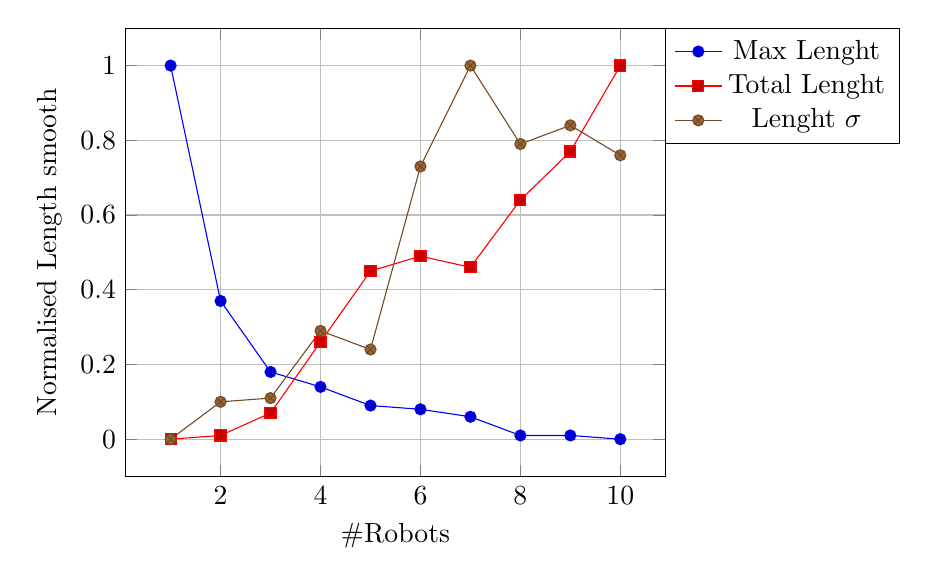
\begin{tikzpicture}
	\begin{axis}[
%		height=9cm,
%		width=9cm,
		grid=major,
                legend style = {at={(1,1)}, anchor=north west},
		xlabel=\#Robots,
		ylabel=Normalised Length
		smooth,
		tension=0.3
	]

	\addplot coordinates {
(1, 1.00)
(2, 0.37)
(3, 0.18)
(4, 0.14)
(5, 0.09)
(6, 0.08)
(7, 0.06)
(8, 0.01)
(9, 0.01)
(10, 0.00)
	};
	\addlegendentry{Max Lenght}

	\addplot coordinates {
(1, 0.00)
(2, 0.01)
(3, 0.07)
(4, 0.26)
(5, 0.45)
(6, 0.49)
(7, 0.46)
(8, 0.64)
(9, 0.77)
(10, 1.00)
	};
	\addlegendentry{Total Lenght}

	\addplot coordinates {
(1, 0.00)
(2, 0.10)
(3, 0.11)
(4, 0.29)
(5, 0.24)
(6, 0.73)
(7, 1.00)
(8, 0.79)
(9, 0.84)
(10, 0.76)
	};
	\addlegendentry{Lenght $\sigma$}
	\end{axis}
\end{tikzpicture}
\caption{Variation of the performance indexes increasing the number of robots, for the 10x10 grid using the VRP with A* algorithm}
\end{figure}